\chapter{General Discussion}
%\chaptermark{Discussion}
\label{ch:discussion}
%\thispagestyle{empty}

Autism and social anxiety each negatively impact one's experiences in communication, language use, and connecting with others \citep{apa2013}. Yet, little is known about how autistic and socially anxious individuals make inferences about the beliefs and thoughts of other people in communicative situations that resemble real-life situations. Even though understanding the neural mechanisms underlying this ability would grant crucial insights on the processes involved, neuroscientific research on this topic using naturalistic task settings is equally scarce. An additional understudied topic concerns linguistic structure building in autistic individuals. In particular, while previous research has investigated spatial differences in neural activation, the temporal dynamics of linguistic structure building in autistic and neurotypical individuals are poorly understood. With three neuroimaging studies involving neurotypical, autistic and socially anxious individuals, we intended to shed new light on these questions. The aims of this thesis were to elucidate the neurocognitive mechanisms underlying mental state inferencing and observing social interactions in autism (chapter~\ref{ch:mentalizing_asc}) and social anxiety (chapter~\ref{ch:mentalizing_sa}), and to investigate the neural signatures of structure building during language comprehension in autistic and neurotypical individuals (chapter~\ref{ch:language_asc}). This general discussion will briefly summarize the findings described in the three empirical chapters, followed by a discussion of how the findings can be integrated with the existing literature. Afterwards, the connection between autism and social anxiety, limitations of the thesis and suggestions for future research will be discussed. 

\section{Summary of findings}

In chapter~\ref{ch:mentalizing_asc}, we aimed to investigate the cognitive mechanisms underlying mental state inferencing in autistic and neurotypical individuals in unpredictable contexts that approximate real-life social interactions. To this end, the neural and pupillary responses in response to a movie featuring social interactions were collected in autistic and neurotypical individuals, after which they both gave verbal descriptions of the movie plot. Comparisons of neural and pupillary responses showed similar processing of movie events that elicited mental state inferences, in addition to similar verbal reasoning about the characters' mental states. Despite this similarity, neural variability computed across the movie was lower for autistic than neurotypical individuals, with the strongest differences occurring outside of mentalizing events and the key mentalizing regions. This points to a more similar way of processing the movie in autistic individuals during the observation of interacting characters. This suggests that the interpretations of these scenes are more consistent among autistic individuals, potentially focusing on similar movie aspects. In chapter~\ref{ch:mentalizing_sa}, our goal was to compare mental state inferencing in individuals with high and low social anxiety within the same, unpredictable context but without eliciting state anxiety coming from explicit task demands. Socially anxious individuals and control participants were tested on similar measures as in chapter~\ref{ch:mentalizing_asc}, in addition to comparing the heart rate of the two groups that gauged their level of state anxiety. Results indicated that the left posterior superior temporal sulcus (pSTS) showed lower neural activation in socially anxious individuals. Neural variability analyses showed brain networks with both heightened and diminished variability in socially anxious individuals compared to control participants. Interestingly, the cluster with the strongest between-group differences in variability showed substantial overlap with the cluster identified in the autism-neurotypical analysis in chapter~\ref{ch:mentalizing_asc}. Importantly, these effects discussed in chapter 3 were elicited amid similar heart rate metrics between the two groups. This indicates that the effects are not due to differences in anxiety experienced during the experiment. These results suggest lower neural activation during mental state inferencing as well as an interpretation bias during social interaction observation. In chapter~\ref{ch:language_asc}, the aim was to assess the neural operations underlying linguistic structure building in autistic and neurotypical individuals, given existing literature indicating aberrant lateralization of language processes. For this reason, we employed EEG to investigate the neural dynamics of linguistic structure building in these populations and how lateralized this process was. An increase in beta power was apparent from the neural signals in both groups when reading sentences compared to reading pseudoword lists. This beta power increase may be interpreted as cognitive maintenance of the ongoing sentence interpretation, and was similar for autistic and neurotypical individuals. Crucially, in a whole-brain and electrode-of-interest analysis, we showed that lateralization of this neural signature of linguistic structure building was similar for the two groups. A regression analysis across the trial time course also showed us that the lateralization stayed the same over the course of the sentence, and that this lateralization time course was similar for both groups. This similar lateralization of the beta power increase indicating linguistic structure building differs from the literature indicating reduced lateralization in autism, mostly with fMRI studies. Nevertheless, these results suggest that not all neural processes underlying language processing are less left-lateralized in autism.  

\section{Insights into communication in autism and social anxiety}
\subsection{Mentalizing in autism}
In chapter~\ref{ch:mentalizing_asc} we observed a similar propensity for mentalizing in neurotypical and autistic individuals with behavioral, pupillary, and neural measures. These novel findings are insightful additions to the current literature because of the more naturalistic and spontaneous way of embedding mentalizing events into a contextually rich narrative compared to many tasks. Furthermore, the movie does not feature linguistic information, which circumvents the problem of testing mentalizing in a population shown to have lower language abilities on average \citep{velikonja2019}. The theory that autistic people in fact have impaired mentalizing ability has permeated psychology for the past 40 years \citep{baron-cohen1985,gernsbacher2019}. This theory suggested that this impairment may be the source of the difficulties they face in everyday social interactions. Against the backdrop of these claims, the absence of mentalizing differences between autistic and neurotypical individuals from chapter~\ref{ch:mentalizing_asc} might seem unexpected. This null effect compared to the effects found in previous mentalizing literature can be explained in several ways. Firstly, the most often used task, the Reading the Mind in the Eyes task (RMET), shows low agreement between different studies using this same task in capturing the same underlying construct \citep{higgins2024}. A recent study even showed that the RMET is more likely to measure emotion recognition instead of mentalizing \citep{oakley2016}. A task with better construct validity might more consistently demonstrate a lack of differences in mental state inferencing in autistic and neurotypical individuals. Secondly, the Partly Cloudy movie bypasses the use of verbal or linguistic utterances in the stimuli, contrary to many other mentalizing tasks. The reliance on language in these tasks may in fact be the source of the differences between autistic and neurotypical individuals, not their mentalizing ability \citep{shaked2006,capage2001,gernsbacher2005,scheeren2013}. Lastly, for the past three decades, a growing number of studies have already demonstrated that not all autistic individuals fail mentalizing tasks. Previous null effects have been observed in metaphor understanding, deception, and verbally reasoning about thoughts and beliefs \citep{happe1993, bowler1992, pantelis2017, vantiel2021, ponnet2005, scheeren2013}. Therefore, the results from chapter~\ref{ch:mentalizing_asc} are in line with this more recent pattern of results. Despite this accumulating evidence demonstrating that a mentalizing deficit is not a universal characteristic of autism, the idea is still widely taught in psychology textbooks \citep{coon2021,kellogg2016,sigelman2018,myers2014}. Science and society would benefit from a more nuanced and realistic picture about mentalizing and autism being taught to the future generations of psychology and psychiatry scientists and clinicians.

\subsection{Mentalizing in social anxiety}
In chapter~\ref{ch:mentalizing_sa}, we discussed that high socially anxious individuals show decreased neural activation in the left pSTS in comparison to low socially anxious individuals when viewing scenes that elicit mental state inferences. This seems to be the first study on the neural mechanisms underlying mentalizing in social anxiety during a non-evaluative setting, informing the several behavioral studies that already exist on this topic. Differential neural activation in the left pSTS suggests that integration of the emotional information in the scenes with the representation of the characters of the narrative happens differently in socially anxious individuals \citep{patel2019,davey2016}. One other study has previously tested mental state reasoning in the socially anxious brain in an economic trust game and found decreased activation in a different brain region, the dorsomedial prefrontal cortex \citep[dmPFC; ][]{sripada2009}. Our approach differs from this study in the improved naturalistic representation of real-life mental state attribution, in the fact that our approach implicitly elicits mental state attribution instead of explicitly, and in showing that the effects are not driven by anxiety, as illustrated by comparable heart rates of both participant groups. Since subtle aspects of mentalizing tasks can influence neural results \citep{schurz2014}, these differences might have contributed to the different location of the observed effects. Specifically, the closer resemblance to real-life social situations compared to the \cite{sripada2009} study may have influenced the process of recognizing emotions and integrating social information into an internal model differently in the socially anxious individuals than the control individuals during the experiment, leading to reduced left pSTS activation. On the behavioral level, we observed that socially anxious individuals were not more inclined to spontaneously reason about mental states when describing the movie plot than controls. Previous studies have found excessive mentalizing performance, that is, overinterpretation of beliefs, for socially anxious individuals in a movie-based task, called the Movie Assessment for Social Cognition \citep[MASC; ][]{hezel2014,washburn2016,dziobek2006}. In this task, participants are asked directly about the feelings and thoughts of characters. This contrasts with our approach, in which we asked participants to only describe the movie plot from which we assessed their propensity to reason with mentalizing-related terms. The MASC has also demonstrated significantly heterogeneous results in comparisons of socially anxious and control participants, most likely due to small sample sizes \citep{baez2023}. The results of the MASC task with these two populations at present might therefore not be fully reliable. In general, it seems that aberrant mentalizing in socially anxious individuals might be more consistent in situations of self-evaluation compared to observing others \citep{ballespi2019}. Future studies investigating whether our behavioral and neural effects hold in situations of self-evaluation will be insightful. Aside from the similar reasoning about mental states, our study also found that socially anxious individuals used fewer negative emotional words when reasoning about the movie plot. This seems in contradiction with evidence showing intact performance on identifying negative emotions in the RMET \citep{washburn2016}. However, the less negative reporting might be a consequence of focusing on not wanting to make a negative impression through their answers. This can be interpreted as a safety behavior from possible negative feedback \citep{wells1995}, consistent with the theory that socially anxious individuals view social situations as minefields for negative evaluations \citep{rapee1997}. 

\subsection{Reduced neural variability in autism}
In chapter~\ref{ch:mentalizing_asc}, we observed that autistic individuals show more correlated neural activation across the movie stimulus than neurotypical individuals. For the first time, this was investigated with an adaptive clustering algorithm that was data-driven across both the temporal and spatial dimension. This finding of increased neural correlation in autistic individuals suggests a different way of interpreting the movie, such as focusing on local, more short-lived information of the movie rather than global information \citep{barnes2012,geelhand2020}. This differential movie interpretation would be consistent with the Weak Central Coherence theory of autism, claiming improved local and reduced global processing of stimuli \citep{happe1997}. However, the reduced variability in autistic participants deviates from the majority of previous studies who found opposite group effects \citep{byrge2015,hasson2009,lyons2020,salmi2013}, indicating more variable neural activation in autistic individuals. This discrepancy in results can be explained by several possible reasons. In contrast to some of the other studies, our movie portrayed anthropomorphic, animated characters instead of real humans. Preliminary evidence indicates that being human or anthropomorphic may influence how much autistic children and adolescents focus on a character's eyes, how approachable they are, as well as their emotion recognition performance \citep{atherton2018}. This could be due to anthropomorphic stimuli often being more exaggerated, making the emotions more intense and overt, and thereby boosting emotion recognition performance in autistic children \citep{carter2016,rump2009}. The between-group differences in our intersubject correlation analysis also deviate from the previously discussed mentalizing-specific analysis showing null effects. The former approach is a data-driven way of analyzing the full duration of the movie, while the latter approach contrasts specific events in the movie. This data-driven correlation approach employs the unpredictable nature of the social interactions of the full movie, compared to existing mentalizing tasks that have less dynamic and more predictable social stimuli. This lack of structure is important to include in our task since real-life social interactions are often unpredictable, ambiguous and messy. For example, when observing a conversation, it is difficult to predict when speakers switch turns and what speakers are about to say. This is similar to the movie used in our task, where the upcoming action or turn in a conversation is hard to predict. The fact that we find group differences to this unpredictable movie is in line with previous research contrasting predictable and unpredictable movie-watching in autistic and neurotypical individuals \citep{roeyers2001,ponnet2008}. In these tasks, two recorded dyadic conversations were viewed by participants and intermittently paused several times to ask about the thoughts of the interlocutors. In both videos, the interlocutors were instructed to get to know each other. Yet, in the first video they were told this was necessary for their performance in a board game they would play later, and they received a list with eight typical `getting acquainted' questions they had to know of one another. In the second video, they did not receive any of these instructions. This influenced the predictability and structure of the two videos. The results indicated that autistic individuals provided less accurate answers on the questions for the unpredictable conversation than neurotypical individuals, showing that they experience more difficulties when viewing unpredictable social stimuli. This approach deviates from our task in that we did not pause to explicitly ask about characters' mental states. Still, it may be the case that the manner in which autistic people attended to information in the Partly Cloudy movie was similar to the manner in which they attended to the conversation videos in \cite{roeyers2001} and \cite{ponnet2008}, and thus might capture part of the difference in task accuracy of the two groups in these two studies. Nevertheless, these findings support the idea that group differences increase when autistic individuals observe or decide on less predictable information. \cite{frith1994} suggest that this pattern of results could be due to autistic individuals relying on non-social heuristics in predictable contexts that do not apply in the unpredictable nature of everyday life, resulting in the difficulties they experience. Furthermore, a general preference for structure is very common in autism \citep{apa2013}, which may result in symptoms of autism being less prominent in predictable contexts \citep{howlin2004,mesibov1992}. 

\subsection{Heightened and reduced neural variability in social anxiety}
In socially anxious individuals, both heightened and diminished neural variability was detected during viewing of social interactions. The more variable brain network comprised of regions involved in processing higher-order information, including the rSMG, ITG, mPFC, the precuneus, while the less variable brain network consisted of lower-order processing regions, such as the superior occipital gyrus and rSTG. This more variable brain network largely overlaps with a previously identified fronto-parietal network showing less activation in socially anxious individuals \citep{koban2023}, indicating differences in attention allocation. Although these data were collected during self-evaluation instead of observing others, the differential strategies might extend to situations in which socially anxious individuals observe others. The variability differences across long segments of the movie might generally indicate a bias of processing and relaying low-level and high-level information. A possible explanation might be that socially anxious individuals have more disparate interpretations of characters' faces or actions, manifesting as more variable high-level processing, which induces more consistent processing of low-level information in a top-down manner. This may be related to interactive behavioral experiments, in which socially anxious individuals seem less conversationally skilled than control individuals in unpredictable conversations \citep{thompson2002,pilkonis1977}. The actions and inferences that the characters make in the movie that we showed are also not very predictable. Therefore, the different interpretations that we pick up on in measuring neural variability might lead to this behavioral deficit presented during unpredictable social interactions. The study we performed was the first of its kind to investigate socially anxious adults. In fact, the bi-directional pattern of neural variability we detected was previously found for socially anxious children, with brain regions showing increased variability overlapping with our results in the frontoparietal cortex \citep{camacho2023}. This increased variability network in social anxiety was also detected in a study with individuals scoring high on a phobia known as Taijin Kyofusho. This culture-specific condition is defined as the fear of embarrassing others through the presentation of one's body or behavior \citep{tei2020}. Contrary to our study, the participants in this study watched videos of people presenting themselves confidently or shamefully while they embarrassed themselves. So, the stimuli did not include dynamic social interactions, but did elicit emotional and mental state inferencing during one-way social interactions. The phobia these participants suffered from is also clinically considered to be more closely related to obsessive compulsive disorder than social anxiety \citep{apa2013}. Thus, while a direct comparison with our study is not possible because of the differences in population and task characteristics, it is promising that these two studies show a brain network in which heightened neural variability is elicited in socially anxious individuals that overlaps with our findings. Taken together, this evidence points to bias in the observation of social stimuli, which has been previously suggested to involve viewing social situations as more threatening or alarming \citep{rapee1997}.

\subsection{Linguistic structure building in autism}
When comparing autistic and neurotypical individuals on electrophysiological measures of linguistic structure building, we observed no differences between the two groups. Contrary to other previously investigated neural markers of linguistic processing, the power increase in the theta, alpha, beta or gamma band during linguistic structure building was not differently lateralized in autistic individuals compared to neurotypical individuals, nor was it left-lateralized in neurotypical individuals in the first place. While previously detected neural signatures of linguistic structure building have been consistently left-lateralized \citep{hagoort2017,giglio2022,fedorenko2010,friederici2003}, most of these studies used fMRI to measure neural activation. Cognitively, this signature may reflect syntactic unification \citep{hagoort2017}. The beta power increase we detected using EEG, is a complementary neural signature to this, and was previously recorded by \cite{bastiaansen2010} and \cite{bastiaansen2015}. This signature may instead reflect the cognitive process of stronger inhibition of bottom-up information in order to maintain a sentence-level representation \citep{miller2018,lewis2016}. The temporal precision of EEG also allowed us to show that the lateralization of structure building did not change over the course of a sentence, neither was this different between groups. These two novel findings add to the understudied topic of the temporal aspect of neural language dynamics, especially in autistic individuals. In sum, our results interact with the existing literature in several ways: they corroborate earlier work on this recently identified neural marker of linguistic structure building, but also show that not all neural mechanisms supporting linguistic processing are lateralized in neurotypical individuals. We also demonstrate that, given the intact behavioral performance, this neural marker does not underlie communication difficulties in autism. The lack of lateralization differences between the two groups calls for nuance when making statements about the commonality of language lateralization differences in autism.

\section{Linking autism and social anxiety}

One might wonder how autism and social anxiety are related given the differences and commonalities we observed in chapter~\ref{ch:mentalizing_asc} and \ref{ch:mentalizing_sa} between autistic and socially anxious participants with respect to neurotypical controls. These results showed a network of brain regions responding more variably in socially anxious individuals and less variably in autistic individuals with respect to controls. While autism and social anxiety are treated and described as distinct \citep{apa2013}, they show overlap in symptoms and common co-occurrence. Social anxiety prevalence among autistic people has been estimated between 21\% and 29\%, in comparison with 4\% to 12\% in neurotypical people \citep{muris1998,simonoff2008,kessler2005,stein2017}. It is suggested that the two conditions often occur together in autistic individuals with average or high cognitive abilities \citep{bellini2004,kuusikko2008}. This finding can be explained by evidence that autistic children with higher intelligence perceive themselves as less socially competent than those with lower intelligence \citep{capps1995}. They are likely more aware of their idiosyncrasies in communication, which generates the downstream consequence of anxiety and avoidance of social situations.

On the one hand, socially anxious behavior in autistic individuals demonstrates similarly to that in non-autistic individuals in some aspects, such as appearing less friendly, avoiding social interactions, impairment in sustaining conversations, and inflexibility \citep{white2011socialanxiety}. On the other hand, socially anxious behavior is different in autistic and non-autistic individuals in terms of the onset of symptoms. The median age of onset of symptoms for social anxiety is 12.5 years and for autism already from 2 years of age \citep{dewit1999,ozonoff2008}. The frequency of initiating social interactions is likely also different between the two populations, since social avoidance is a hallmark of social anxiety but social initiation is not necessarily impaired in autism \citep{white2011socialanxiety,humphrey2011}. Research on the neural mechanisms that underlie the differences between social anxiety in autistic and non-autistic individuals is limited. By using an emotional identification task, one study by \cite{kleinhans2010} showed that activation in the right amygdala, left MTG, and fusiform face area was correlated with social anxiety scores in autistic, but not in non-autistic individuals. This suggests that social anxiety in the two populations has different underlying sources. This is in line with the idea of social anxiety being a consequence of autistic behavior, but not a core symptom.

From behavioral experiments, we know that both socially anxious and autistic individuals struggle most in unpredictable social interactions. For this type of interactions, autistic individuals' reasoning about mental states is less accurate and socially anxious individuals' conversational skills are impaired \citep{roeyers2001,ponnet2008,pilkonis1977,thompson2002}. This similarity is relevant for the results discussed in chapter~\ref{ch:mentalizing_asc} and \ref{ch:mentalizing_sa} because of the unpredictable quality of the narrative, the actions and the inferences featured in the Partly Cloudy movie. However, the neural variability findings we discussed in chapter~\ref{ch:mentalizing_sa} likely do not explain the network showing opposite variability for autistic and socially anxious individuals. While the neural regions of the variability effect in the two groups overlap, the variability differs in the opposite direction for the groups: socially anxious individuals show higher variability vs. autistic individuals show lower variability compared to controls. Therefore, an opposite effect does not match the similarly lower behavioral performance in both groups with respect to controls in unpredictable conversations.

It appears that the discussed similarities and differences of social anxiety occurring with or without autism do not explain the pattern of the neural variability findings we discussed in chapter~\ref{ch:mentalizing_sa}. There, we found that the same neural network showed variability of the opposite magnitude for autistic and socially anxious individuals. This finding is the first of its kind in the domain of neural processes, though it has already been encountered in eye-tracking studies. These experiments showed that autistic individuals orient their gaze towards eyes with a delay compared to controls, while socially anxious individuals orient faster towards eyes and subsequently look away \citep{ni2023,kleberg2017}. These low-level differences could perhaps cause the previously discussed differences in social behavior between social anxiety and autism. Future studies on neural variability in these two populations using different stimuli or tasks might inform on which aspects the two conditions overlap and why.

\section{Limitations}

The research discussed in chapter~\ref{ch:mentalizing_asc} to \ref{ch:language_asc} has several limitations to be discussed. Firstly, the individuals who took part in our experiments were of average to high intelligence (average verbal IQ was 126 and non-verbal IQ was 103). This limits the ways in which we can generalize our findings to individuals with lower IQ. This is especially pertinent for autistic individuals, of whom an estimated 33\% to 50\% has an intellectual disability \citep{katusic2021,shenouda2023}. Our participants were also highly verbal, as almost all were able to talk fluently about abstract topics during test sessions. This contrasts with the experiences of many autistic adults, since 30\% of autistic individuals are non-verbal and their language ability is on average 1.5 standard deviation lower than neurotypical individuals \citep{kwok2015,anderson2007}. One could suggest to extrapolate the effects of our autistic participants to lower IQ scores. Yet, autistic participants with more support needs can show qualitatively different behavior, which makes a linear extrapolation not useful \citep{wenar1986}. Despite the sampling bias of the autistic individuals, we can still state that the null effects found in chapter~\ref{ch:mentalizing_asc} and \ref{ch:language_asc} suggest the absence of a universal effect across the autism spectrum.

Furthermore, while our use of a movie featuring dynamic social interactions is more naturalistic than many structured and static mentalizing tasks, the movie we showed participants features animated, anthropomorphic characters, background music, and fantastical elements. Because of these aspects, our results cannot be directly generalized to the observations of real-life social interactions. Moreover, each movie has its own unique storyline and characters. It will be important to assess whether movies featuring different topics, characters, and plot will elicit similar results. Using movies featuring humans involved in various types of realistic social interactions as stimuli will provide additional integral insights into understanding mental state inferencing and social cognition.

\section{The way forward for mentalizing research}

With the research conducted in chapters~\ref{ch:mentalizing_asc} to \ref{ch:mentalizing_sa}, we have shown that mentalizing embedded in the observation of naturalistic interactions engages key regions of the mentalizing network. This teaches us that the neural processes that we expect to occur during less naturalistic mentalizing hold up and scale up to more naturalistic situations. Yet, our understanding of the neural mechanisms supporting the inferences of someone's mental state is still limited. The following section will outline several practices and lines of research that I believe will contribute substantially to the understanding of how people come to understand the thoughts and beliefs of others.

A simple advancement of the field would be to improve and standardize the terminology. For example, "cognitive" and "affective" mentalizing have been introduced a few decades ago to provide more specification to the term \citep{brothers1992,shamay2009}. However, the processes involved in these two constructs are still not well explained, and alternative terms with the same meaning exist. In the field of mentalizing, we often encounter the use of the same terms to refer to different constructs (such as theory of mind or empathy) and of different terms to refer to the same construct (such as theory of mind, mentalizing, mindreading). This obstructs comparing and generalizing research, as "implicit in the vocabulary are a surprising number of theoretical claims" \citep[p. 14]{searle1992}. In their large survey on researchers in the field of mentalizing, \cite{quesque2024} show that researchers are willing to discontinue terms, and, although no unanimous agreement could be reached, a large majority agreed on a common lexicon of terms related to mental state attribution. They propose "mentalizing" as the common term to refer to "the ability to attribute mental states (e.g., knowledge, intentions, emotions, perception) to self and others" \citep[p. 2]{quesque2024}, which is a felicitous term for the construct that the field can collectively use. 

Another way of increasing naturalism and fidelity of mental state inferencing studies, is to more explicitly take into account the mental state that is being inferenced \citep{conway2019}. Consider the classic Sally-Anne task, in which the character Sally puts her ball in a basket, leaves the room, after which the character Anne moves the ball to a box. Sally then comes back and the participant is asked where Sally will look for her ball. In the original version, where the participant has no information about Sally, they will most likely answer "the basket", that is, the place where she left it. Yet, in a situation where we know Sally is a highly suspicious person, a participant could be more likely to assume Sally to first look at the box, being more inclined to believe that Anne has moved her precious ball. In the real world, we often have information about traits such as suspiciousness or forgetfulness, or about moods such as being happy or depressed, or about the cultural background of our communicative partner, which may all influence the mental state we infer of them. Information about age, for example, influences if and how we adjust our communication to the other person, like for instance the tendency to speak slower to elderly because we suspect that their processing speed might not keep up with our normal speech rate \citep{stolk2013neural,kemper1999}. These trait characteristics are also relevant for interpreting the Partly Cloudy movie from chapter~\ref{ch:mentalizing_asc} and ~\ref{ch:mentalizing_sa}: through the different scenes in the movie we come to know one of the main characters as suspicious, which affect subsequent inferences of their mental state. For these reasons, the facets and traits of a mind are crucial for good models of attributing a mental state to the same mind. 

This representation of facets and traits of a mind is a subcomponent of mentalizing. In fact, breaking mentalizing into its subcomponents \citep["deconstructing" it;][]{schaafsma2015} is a necessary step to gain a better understanding of the mechanisms involved. Showing higher neural activation in some brain region in response to a broad mentalizing task or stimulus is after all a somewhat underspecified model of the process. \cite{schaafsma2015} present a non-exhaustive list of subcomponents of mentalizing that includes, among other aspects, face recognition, which is necessary for emotion processing, which is in turn necessary for inferring mental states from eyes. This idea of deconstruction would be more effective and concrete if it could be applied to specific instances of mental state inferencing. For this reason, and to put findings of chapter~\ref{ch:mentalizing_asc} and ~\ref{ch:mentalizing_sa} more in perspective, I will summarize and deconstruct one of the mental events in the Partly Cloudy movie of the task in order to characterize the cognitive processes necessary for mental state inferencing during action observation.  

The Partly Cloudy movie centers around the interactions between two main characters: a grey cloud and a stork. It is set in a world where clouds create baby animals and humans, and storks collect them from these clouds and deliver them to the happy parents. The critical moment during one of the mental events happens when the main cloud character gets angry, which is when the viewer is meant to infer their mental state on the basis of, among other things, the preceding context in the narrative. This context includes the fact that, firstly, during the narrative the main cloud character has only created dangerous or painful baby animals, like a hedgehog and an alligator, that attack the stork while carrying them. During these moments, we see that the cloud sees his friend getting hurt and that the cloud has a facial expression of worry. From this, we can infer that the cloud is worried about the stork getting hurt. Secondly, the context includes a scene when the main stork looks at a brighter, more colorful looking cloud that creates friendlier and cuter creatures than his own cloud has created. We see the stork looking at this cloud with a happy facial expression and upon seeing the stork looking at the other cloud, the grey cloud has a sad and worried facial expression. After that, we see that the stork notices the cloud's worried look and acts like he was not looking at the other cloud. From this scene, we can infer two things: the cloud is worried about the stork being envious about other clouds offering friendlier creatures, and stork is concerned with not looking envious in front of the other cloud. The context of the movie just before the critical mental-state-inferencing moment happens as follows: the grey cloud creates a new package for the stork to carry, in the shape of a shark, after which the cloud sees that the stork sees that a different, brighter cloud has created friendly animals again. Upon seeing this potentially deadly creature in the cloud's hands and having seen the friendlier creatures at a different cloud, the stork flies away to the cloud with the friendlier animals. These are the narrative context and inferences necessary to infer the mental reasoning of the angry cloud, which is most commonly reported by participants as: the cloud is unhappy because he thinks that the stork has betrayed him.  

With this description of information necessary for inferring this specific mental state, we can consider which cognitive processes are involved. Evidently, one first needs systems that provide access to the visual and auditory input to these scenes. Within these scenes, it is important to track which information is available or visible to which characters and additionally whether that viewpoint differs from our own viewpoint, known as `self-other distinction' \citep{quesque2020}. In the movie, the grey cloud has access to the same visual information as the viewer. Yet, the cloud looks more worried than the viewer is likely to be, because of the stork's dedication to their friendship and the faith that the stork will therefore not leave the cloud. Encoding and retrieval processes are crucial for this tracking of viewpoints of characters, in addition to other bits of short-term and long-term information such as memories and learned associations. An example of relevant short-term information here would be to remember that the cloud is likely to worry about the stork's envy. Relevant long-term information, learned by the viewer well before watching the movie, would be that furrowed eyebrows and downward facing corners of the mouth are associated with feeling sad. Clearly, associations like this are important since they are the basis for emotion recognition. Lastly, essential to the ability to reason about the angry cloud's mental state is the ability to understand causality and the fact that characters act according to their goals and desires. This is especially important when seeing the stork fly away from the grey cloud, as this happens right after the grey cloud offers the stork a shark-shaped package and the stork sees much friendlier creatures being created at a different cloud. Being able to causally link these actions to subsequent actions allows the viewer to be able to understand the angry cloud.

With these cognitive processes laid out, we might be able to examine the results of chapter~\ref{ch:mentalizing_asc} and ~\ref{ch:mentalizing_sa} in a bit more detail. While neurotypical and autistic individuals showed similar neural activation during mentalizing, socially anxious individuals showed lower activation in the left pSTS in comparison to neurotypical individuals. Since the left pSTS is typically involved in recognizing emotions and integrating social information into an internal model \citep{peelen2010,samson2004}, it is possible that encoding (negative) emotions or facial expressions is diminished in socially anxious individuals. A second possibility is a diminished self-other distinction, blurring the line between themselves and the character on screen due to lower pSTS activation. We can also consider the neural variability findings again, which are based on analyses taking the full movie into account. While these data are not made up of exclusively strictly mentalizing events, many of the same cognitive operations are necessary to interpret social observations in general. As discussed, these findings showed a network of brain regions showing higher variability in socially anxious individuals and lower variability in autistic individuals compared to neurotypical individuals. Given the previously found pattern in eye-tracking research \citep{kleberg2017,ni2023}, the network could be sensitive to encoding gaze processing and functionally related to a frontal parietal attention network detected in other studies \citep{camacho2023,koban2023,tei2020}. We also detected a network showing lower variability in socially anxious compared to neurotypical individuals, possibly regulating the encoding of lower-level sensory information from characters' faces, bodies and sounds given its location in the primary visual and auditory cortex. Altogether, making the operations involved in mentalizing and social observation more explicit, allows us to interpret the findings more thoroughly and deeply. 

The described overview of cognitive processes now gives us an idea of the elements and operations involved in mental state inferencing: processing of several streams of input, storage of long- and short-term information and architecture that can link representations. In real life, an additional component would be the metacognitive capacity to evaluate the certainty of bits of memory and input. Taken together, these components provide a foundation from which to start building computational models of mental state inferencing. Computational models are a crucial part of psychology and neuroscience because they can provide information about the causal influence of an operation on the output through simulation \citep{guest2020}. This is in contrast to empirical testing with neuroimaging, which, while useful, can only provide evidence of correlational nature. Computational models additionally require formally defining a theory, removing its ambiguity and improving its falsifiability \citep{guest2021}. These theories can be built starting from an established element at the functional level \citep[or computational level;][]{marr1982}, where the goal of the system is described. An example from language comprehension of such an element might be hearing and processing a distinctive feature \citep[the most basic unit in phonology;][]{poeppel2005}. For mental state attribution, it could be seeing and processing a facial feature. The "Bayesian Mentalizing" model is an example of a model built from the functional level, in which the actions of a rational agent choosing between food options were simulated based on inverse modelling of a partially observable Markov decision process \citep{baker2017}. While model performance was strongly correlated with behavioral data, the highly-simplified model was still computationally intractable, that is, not computable in a time frame reasonably expected from human cognition. A more realistically grounded approach would be to start modelling at the implementational level, where the hardware of the system is described \citep{fitz2024}. In these neurobiological causal models, functional equations are designed that describe a system from first principles in neurobiology. Crucially, these models surpass functional-first models in that they provide a clear association to the implementational substrate. The feasibility and usefulness of neurobiologically constrained models have already been demonstrated in the domain of learning abstract and concrete words \citep{dobler2024}. Building a neurobiological causal model of mental state attribution will be require a great deal of time and effort given the multi-faceted nature of a real-life mental state inference. Nevertheless, the subsequent contributions will provide invaluable insights into the neural mechanisms of mental state inferencing.  

\section{Putting language in context: the Neuro-Crime Scene Investigation paradigm}

The research covered in this thesis has addressed the neural mechanisms underlying linguistic structure building (chapter~\ref{ch:language_asc}) and mentalizing (chapter~\ref{ch:mentalizing_asc} and ~\ref{ch:mentalizing_sa}) in autistic people. This aids our understanding of the underlying operations during, on the one hand, interpreting the literal meaning of utterances and, on the other hand, inferencing about the mental states of others. These capacities are the building blocks of communication, and they often work together to help us understand the meaning of an utterance \citep{basnakova2014beyond,ferstl2008,Xu2005}. This collaborative operation is necessary to understand language when meaning is strongly dependent on the context it appears in. This often occurs in real-life dialogue: consider the meaning of the word bank if it is spoken in the context of a conversation about investments or about rivers. Similarly, the remark "Great job" during a game of baseball can be either sincere or sarcastic depending on whether the player just hit a foul ball or a home run. Several different lines of research have shown that autistic individuals tend to struggle with context-dependent language use \citep{angeleri2016,loukusa2007,wadge2019}. These effects are in contrast with the null findings between autistic and neurotypical groups in mentalizing and linguistic structure building reported in this thesis. These demonstrated effects on context-dependent language understanding therefore warrant more discussion and consideration about how this crucial communication skill can be optimally tested.

The way in which autistic people struggle with context-dependent language has been demonstrated in several experiments using homographs \citep{jolliffe1999,happe1997,frith1983,eberhardt2018,hahn2015,brock2008}. In these experiments, autistic and neurotypical children with similar reading ability are asked to read aloud sentences with target words that have two different interpretations and pronunciations. For example, the word tear is pronounced differently for a context-appropriate interpretation in the sentence "In her eye/dress is a big tear", depending on the words in the context. Several studies have shown that autistic individuals apply the context-inappropriate pronunciation more often than neurotypical individuals \citep{jolliffe1999,happe1997,frith1983}, although recent findings are more mixed \citep{eberhardt2018,hahn2015,brock2008}. Diminished metaphor and irony understanding as well as atypical strategies in understanding non-literal language have also been observed in autistic individuals \citep{pexman2011,rundblad2010,deliens2018}. Many of these studies, however, only use one or two sentences as context in their experiment, while everyday conversations are typically much richer in discourse context. The underlying neurocognitive processes of inferring and integrating context are also relatively unknown. The current evidence points to involvement of the right inferior frontal gyrus (RIFG) during integrating speaker information with the current linguistic utterance and during irony comprehension \citep{tesink2009neural,wang2006}. Whether these findings also hold for integrating a dialogue-like linguistic discourse context with the current linguistic utterance is an open question. 

Originally, as part of the plan of the current thesis, we designed and ran a study that combined mentalizing and linguistic processing in one neuroimaging experiment investigating contextual language interpretation. Due to time constraints and delays as a consequence of the COVID-19 pandemic, it was not possible for me to include the results and finished manuscript in the current thesis. The design of this prospective experiment, however, is still relevant for the current discussion on studying the neurocognitive mechanisms underlying communication. Therefore, I will briefly describe the paradigm and its potential contribution to the field.
 
To study the use of a dialogue context in language comprehension, we developed a new experimental paradigm, called the NeuroCSI (Neuro-Crime Scene Investigation; see Fig~\ref{fig:csi}). In this fMRI paradigm, participants were asked to play the part of an investigator who is hired by the FBI to check chat conversations to see if the interlocutors are discussing criminal activities. The back-and-forth dialogue stimuli were chosen to emulate social interaction, while preserving tractability over the stimuli. While reading these conversations in the MRI scanner, the participants were led to build an internal situation model, that is, a mental representation of the situation described by the interlocutors in the messages. For half of the dialogues, the target word was a slang word, for example `bears' meaning `police'. By reading the sentences one by one, they would infer the slang meaning based on the accumulating contextual information present in the dialogue. For the other half of the dialogues, the target word did not have a slang meaning, but was used in its literal meaning. By contrasting these two types of dialogues, we were able to manipulate a change in interpretation over the time it takes to read the dialogue and measure the corresponding cognitive processes. The first sentence that could indicate that the target word has a slang meaning was labelled the `expectation violation' sentence. From this sentence onwards, the participants should notice the change in meaning and gradually adjust their situation model, which was measured with fMRI. In this study, autistic and neurotypical individuals matched on age and verbal IQ have been included. 
\begin{figure}[!h]
	\centering
	\hspace*{-0.7cm}
	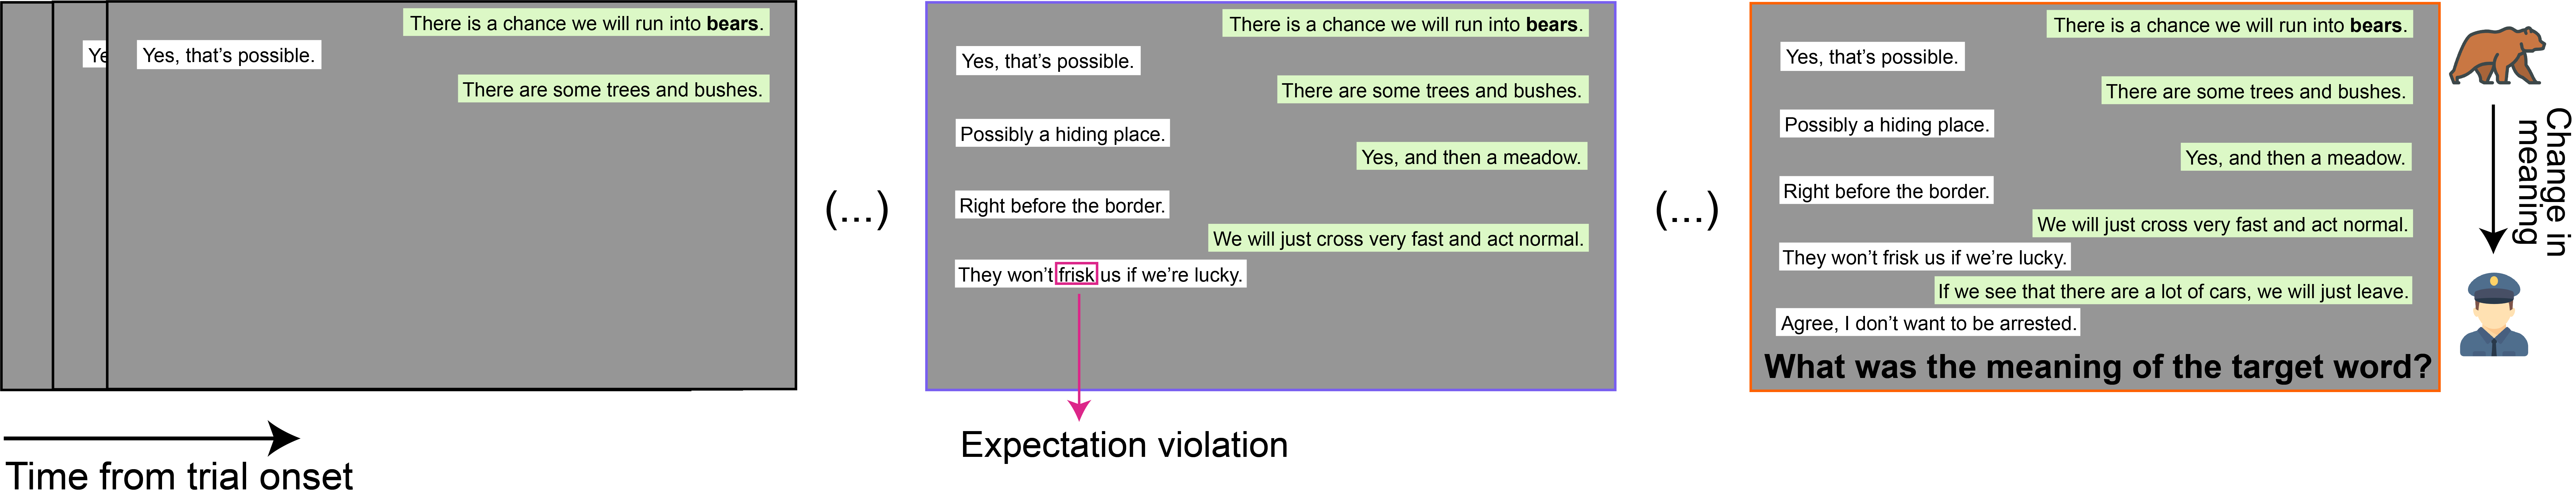
\includegraphics[width=1.1\textwidth, clip=true]{./Chapters/05_Discussion/Images/csi_image_horizontal}
	\caption{The NeuroCSI paradigm, which aims to probe the cognitive processes underlying the integration of context with utterance meaning. Participants read the chat conversation for which sentences appear on screen one at a time. In this example trial, the target word (\textit{bears}) has a different meaning (\textit{police}) than its literal meaning. The first sentence that could indicate that the target word has a slang meaning is the \textit{expectation violation} (see screen with purple outline), a critical event for analysis. After all sentences have appeared on screen, the participants decide on the meaning of the target word (see screen with orange outline). In these "slang" trials, the likely meaning of the target word has changed from its literal meaning to the slang meaning over the course of the dialogue and can be inferred from the context. }
    \vspace*{-10pt}
	\label{fig:csi}
\end{figure}

The design of this study uniquely combines language comprehension and mentalizing. On the one hand, participants have to make sense of the literal meaning of the messages in the dialogue and integrate each message with the unfolding context. On the other hand, when the literal meaning seems unlikely to fit the context, they must imagine what the interlocutors might mean with a possible slang target word. Based on the results in chapter~\ref{ch:language_asc}, I hypothesize that autistic and neurotypical people might perform equally well in trials where the intended meaning by the interlocutor matches the literal meaning. However, the decreased neural variability in autistic participants discussed in chapter~\ref{ch:mentalizing_asc} suggest that autistic individuals may focus more on the literal meaning of the dialogue and therefore show weaker or delayed integration of the intended meaning. The results of this upcoming study alongside those of the other chapters in this thesis will inform behavioral and neural theories on how autistic individuals integrate linguistic and social information into the interpretation of a signal \citep{wadge2019}. Difficulties in social interactions like context-inappropriate language use commonly influence connections and friendships for autistic people \citep{howlin2004,bauminger2003,bauminger2000}. For this reason, understanding the cognitive mechanisms underlying autistic communication is necessary to improve their well-being.

\section{Solving the puzzle of communication}

In chapters \ref{ch:mentalizing_asc} to \ref{ch:language_asc}, I have outlined experiments on mental state inferencing and linguistic structure building. While these are undeniably crucial pieces to solving the puzzle of communication, the single-person approach in which these experiments were conducted can only tell us so much about communication, an activity typically involving more than one person. This is for instance demonstrated by the finding that simply having another person present in a non-communicative task can affect a principal psycholinguistic process like lexical retrieval \citep{kuhlen2017having}. To see if these psycholinguistic and psychological abilities hold up in situations where more people are present, replicating these studies in a set-up with more than one person is important to validate the ecological validity of their effects.

A big part of the puzzle may be solved with new insights into communication in interactive settings. Psychology and language have primarily investigated their respective phenomena with participants engaging in a one-way interpretation of utterances or signals. This gives a one-sided view of the mind, since we acquire interests, fears, desires, and the meaning of concepts through others \citep{zaki2011,safran2014,defelice2023}. As briefly mentioned in chapter~\ref{ch:introduction}, understanding the dynamic, back-and-forth nature of communication calls for more insight into, firstly, the creative way in which interlocutors can create and use referents and words in dialogue. Introducing and using newly created terms to refer to people and objects can help define and clear up ideas, and in turn make sure you and the person you are speaking to are talking about the same thing or person \citep{brennan1996}. For example, if you have two friends named Alex, you might refer to one or both of them with a distinctive feature, like what they study, and call them \textit{Walex} (\underline{w}iskunde = mathematics) and \textit{Skalex} (\underline{s}cheikunde = chemistry). This process of reference creation and use is known as entrainment in the psycholinguistic literature \citep{brennan2010}. Preliminary evidence suggests that the right temporal lobe and ventromedial PFC are involved in producing and interpreting these new signals \citep{stolk2013neural}. To the same end, it is not just important what to say but also when to say it: responding in a timely manner is important for an enjoyable conversation and feelings of social connection with your conversational partner \citep{templeton2022}. Even more so, poorly timed responses carry (unintended) meaning. Think of a `no' uttered very fast in response to an invitation, which can come off as rude, or the exact opposite, a `yes' uttered slowly, possibly indicating unwillingness to accept a request \citep{bogels2015never,kendrick2015}. The existing neuroscientific evidence shows that this response planning starts already 500 ms after hearing the critical information in the conversation partner's utterance \citep{bogels2015neural}. These subtle and fleeting pieces of the communication puzzle show the mounting complexity of the problem in interactive settings and therefore warrant more investigation. 

Understanding the interactive aspect of communication is all the more important in autism and social anxiety, since the difficulties and frustrations of these individuals arise from interactive settings. Since autistic and socially anxious individuals struggle the most in unpredictable conversations \citep{roeyers2001,ponnet2008,pilkonis1977,thompson2002}, the most valuable insights are to be gained from experiments in unpredictable, interactive settings paired with tools to measure the underlying neural mechanisms of fleeting conversational dynamics. 

\section{Conclusion}

This thesis has described the neural mechanisms underlying mental state inferencing and language comprehension in autism and social anxiety. By examining mental state inferencing in a more naturalistic context our findings indicate, on the one hand, that autistic and neurotypical individuals have similar behavioral and neural responses. On the other hand, differences between the two groups are elicited in their neural variability in response to viewing social interactions. When comparing socially anxious and control participants in this way, decreased neural activation during mental state inferencing is found for socially anxious individuals in addition to differences in neural variability. Crucially, these differences were not due to anxiety during the experiment. When examining neural signatures of linguistic structure building, autistic and neurotypical individuals show similar neural measures on a reliably identified oscillatory component, as well as similar lateralization of this component. These insights indicate that the use of experimental set-ups that approximate everyday situations is a promising way of learning more about how neurotypical and neurodivergent understand language and communication. 